% This file is generated by the MATLAB m-file laprint.m. It can be included
% into LaTeX documents using the packages graphicx, color and psfrag.
% It is accompanied by a postscript file. A sample LaTeX file is:
%    \documentclass{article}\usepackage{graphicx,color,psfrag}
%    \begin{document}% This file is generated by the MATLAB m-file laprint.m. It can be included
% into LaTeX documents using the packages graphicx, color and psfrag.
% It is accompanied by a postscript file. A sample LaTeX file is:
%    \documentclass{article}\usepackage{graphicx,color,psfrag}
%    \begin{document}% This file is generated by the MATLAB m-file laprint.m. It can be included
% into LaTeX documents using the packages graphicx, color and psfrag.
% It is accompanied by a postscript file. A sample LaTeX file is:
%    \documentclass{article}\usepackage{graphicx,color,psfrag}
%    \begin{document}% This file is generated by the MATLAB m-file laprint.m. It can be included
% into LaTeX documents using the packages graphicx, color and psfrag.
% It is accompanied by a postscript file. A sample LaTeX file is:
%    \documentclass{article}\usepackage{graphicx,color,psfrag}
%    \begin{document}\input{Psaltis_plot}\end{document}
% See http://www.mathworks.de/matlabcentral/fileexchange/loadFile.do?objectId=4638
% for recent versions of laprint.m.
%
% created by:           LaPrint version 3.16 (13.9.2004)
% created on:           31-Jul-2013 16:31:14
% eps bounding box:     15 cm x 11.25 cm
% comment:              
%
\begin{psfrags}%
\psfragscanon%
%
% text strings:
\psfrag{s03}[l][l]{\color[rgb]{0.83529,0.36863,0}\setlength{\tabcolsep}{0pt}\begin{tabular}{l}$10^6 M_\odot$\end{tabular}}%
\psfrag{s04}[l][l]{\color[rgb]{0.83529,0.36863,0}\setlength{\tabcolsep}{0pt}\begin{tabular}{l}$M_\odot$\end{tabular}}%
\psfrag{s05}[l][l]{\color[rgb]{0.83529,0.36863,0}\setlength{\tabcolsep}{0pt}\begin{tabular}{l}$M_\oplus$\end{tabular}}%
\psfrag{s06}[l][l]{\color[rgb]{0,0.44706,0.69804}\setlength{\tabcolsep}{0pt}\begin{tabular}{l}$1~\mathrm{m}$\end{tabular}}%
\psfrag{s07}[l][l]{\color[rgb]{0,0.44706,0.69804}\setlength{\tabcolsep}{0pt}\begin{tabular}{l}$10~\mathrm{km}$\end{tabular}}%
\psfrag{s08}[l][l]{\color[rgb]{0,0.44706,0.69804}\setlength{\tabcolsep}{0pt}\begin{tabular}{l}$1 R_\oplus$\end{tabular}}%
\psfrag{s09}[l][l]{\color[rgb]{0,0.44706,0.69804}\setlength{\tabcolsep}{0pt}\begin{tabular}{l}$1 R_\odot$\end{tabular}}%
\psfrag{s10}[l][l]{\color[rgb]{0,0.44706,0.69804}\setlength{\tabcolsep}{0pt}\begin{tabular}{l}$1~\mathrm{mpc}$\end{tabular}}%
\psfrag{s11}[l][l]{\color[rgb]{0,0,0}\setlength{\tabcolsep}{0pt}\begin{tabular}{l}GP-B\end{tabular}}%
\psfrag{s12}[l][l]{\color[rgb]{0,0,0}\setlength{\tabcolsep}{0pt}\begin{tabular}{l}LLR (Earth--Moon)\end{tabular}}%
\psfrag{s13}[l][l]{\color[rgb]{0,0,0}\setlength{\tabcolsep}{0pt}\begin{tabular}{l}LLR (Earth--Moon--Sun)\end{tabular}}%
\psfrag{s14}[l][l]{\color[rgb]{0,0,0}\setlength{\tabcolsep}{0pt}\begin{tabular}{l}Mercury\end{tabular}}%
\psfrag{s15}[l][l]{\color[rgb]{0,0,0}\setlength{\tabcolsep}{0pt}\begin{tabular}{l}Cassini\end{tabular}}%
\psfrag{s16}[l][l]{\color[rgb]{0,0,0}\setlength{\tabcolsep}{0pt}\begin{tabular}{l}Hulse--Taylor\end{tabular}}%
\psfrag{s17}[l][l]{\color[rgb]{0,0,0}\setlength{\tabcolsep}{0pt}\begin{tabular}{l}J0348+0432\end{tabular}}%
\psfrag{s18}[l][l]{\color[rgb]{0,0,0}\setlength{\tabcolsep}{0pt}\begin{tabular}{l}Double pulsar\end{tabular}}%
\psfrag{s19}[l][l]{\color[rgb]{0,0,0}\setlength{\tabcolsep}{0pt}\begin{tabular}{l}Neutron star\end{tabular}}%
\psfrag{s20}[l][l]{\color[rgb]{0,0,0}\setlength{\tabcolsep}{0pt}\begin{tabular}{l}Black holes\end{tabular}}%
\psfrag{s21}[t][t]{\color[rgb]{0,0,0}\setlength{\tabcolsep}{0pt}\begin{tabular}{c}{\Large{$\xi/\mathrm{m^{-2}}$}}\end{tabular}}%
\psfrag{s22}[b][b]{\color[rgb]{0,0,0}\setlength{\tabcolsep}{0pt}\begin{tabular}{c}{\Large{$\varepsilon$}}\end{tabular}}%
%
% xticklabels:
\psfrag{x01}[t][t]{$10^{-30}$}%
\psfrag{x02}[t][t]{$10^{-25}$}%
\psfrag{x03}[t][t]{$10^{-20}$}%
\psfrag{x04}[t][t]{$10^{-15}$}%
\psfrag{x05}[t][t]{$10^{-10}$}%
%
% yticklabels:
\psfrag{v01}[r][r]{$10^{-12}$}%
\psfrag{v02}[r][r]{$10^{-10}$}%
\psfrag{v03}[r][r]{$10^{-8}$}%
\psfrag{v04}[r][r]{$10^{-6}$}%
\psfrag{v05}[r][r]{$10^{-4}$}%
\psfrag{v06}[r][r]{$10^{-2}$}%
\psfrag{v07}[r][r]{$10^{0}$}%
%
% Figure:
\resizebox{12cm}{!}{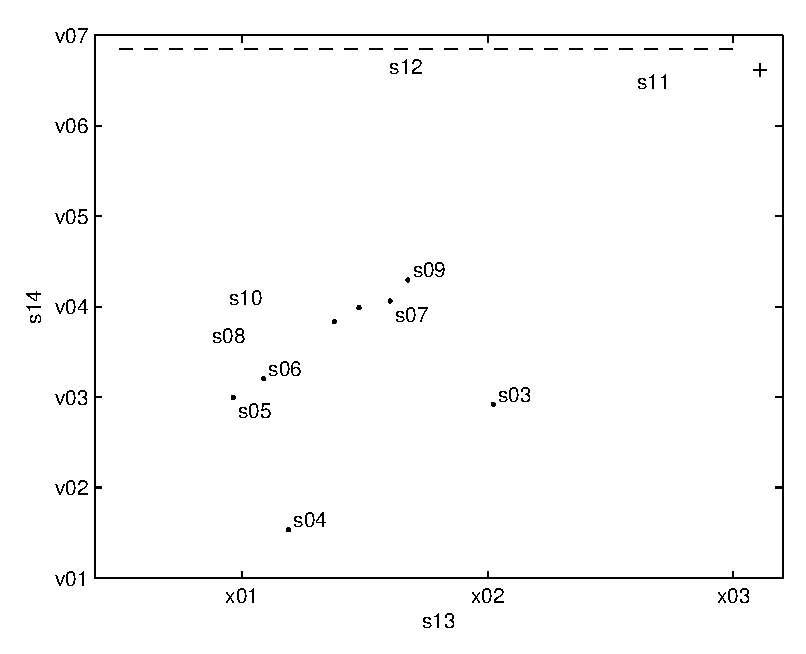
\includegraphics{Psaltis_plot.eps}}%
\end{psfrags}%
%
% End Psaltis_plot.tex
\end{document}
% See http://www.mathworks.de/matlabcentral/fileexchange/loadFile.do?objectId=4638
% for recent versions of laprint.m.
%
% created by:           LaPrint version 3.16 (13.9.2004)
% created on:           31-Jul-2013 16:31:14
% eps bounding box:     15 cm x 11.25 cm
% comment:              
%
\begin{psfrags}%
\psfragscanon%
%
% text strings:
\psfrag{s03}[l][l]{\color[rgb]{0.83529,0.36863,0}\setlength{\tabcolsep}{0pt}\begin{tabular}{l}$10^6 M_\odot$\end{tabular}}%
\psfrag{s04}[l][l]{\color[rgb]{0.83529,0.36863,0}\setlength{\tabcolsep}{0pt}\begin{tabular}{l}$M_\odot$\end{tabular}}%
\psfrag{s05}[l][l]{\color[rgb]{0.83529,0.36863,0}\setlength{\tabcolsep}{0pt}\begin{tabular}{l}$M_\oplus$\end{tabular}}%
\psfrag{s06}[l][l]{\color[rgb]{0,0.44706,0.69804}\setlength{\tabcolsep}{0pt}\begin{tabular}{l}$1~\mathrm{m}$\end{tabular}}%
\psfrag{s07}[l][l]{\color[rgb]{0,0.44706,0.69804}\setlength{\tabcolsep}{0pt}\begin{tabular}{l}$10~\mathrm{km}$\end{tabular}}%
\psfrag{s08}[l][l]{\color[rgb]{0,0.44706,0.69804}\setlength{\tabcolsep}{0pt}\begin{tabular}{l}$1 R_\oplus$\end{tabular}}%
\psfrag{s09}[l][l]{\color[rgb]{0,0.44706,0.69804}\setlength{\tabcolsep}{0pt}\begin{tabular}{l}$1 R_\odot$\end{tabular}}%
\psfrag{s10}[l][l]{\color[rgb]{0,0.44706,0.69804}\setlength{\tabcolsep}{0pt}\begin{tabular}{l}$1~\mathrm{mpc}$\end{tabular}}%
\psfrag{s11}[l][l]{\color[rgb]{0,0,0}\setlength{\tabcolsep}{0pt}\begin{tabular}{l}GP-B\end{tabular}}%
\psfrag{s12}[l][l]{\color[rgb]{0,0,0}\setlength{\tabcolsep}{0pt}\begin{tabular}{l}LLR (Earth--Moon)\end{tabular}}%
\psfrag{s13}[l][l]{\color[rgb]{0,0,0}\setlength{\tabcolsep}{0pt}\begin{tabular}{l}LLR (Earth--Moon--Sun)\end{tabular}}%
\psfrag{s14}[l][l]{\color[rgb]{0,0,0}\setlength{\tabcolsep}{0pt}\begin{tabular}{l}Mercury\end{tabular}}%
\psfrag{s15}[l][l]{\color[rgb]{0,0,0}\setlength{\tabcolsep}{0pt}\begin{tabular}{l}Cassini\end{tabular}}%
\psfrag{s16}[l][l]{\color[rgb]{0,0,0}\setlength{\tabcolsep}{0pt}\begin{tabular}{l}Hulse--Taylor\end{tabular}}%
\psfrag{s17}[l][l]{\color[rgb]{0,0,0}\setlength{\tabcolsep}{0pt}\begin{tabular}{l}J0348+0432\end{tabular}}%
\psfrag{s18}[l][l]{\color[rgb]{0,0,0}\setlength{\tabcolsep}{0pt}\begin{tabular}{l}Double pulsar\end{tabular}}%
\psfrag{s19}[l][l]{\color[rgb]{0,0,0}\setlength{\tabcolsep}{0pt}\begin{tabular}{l}Neutron star\end{tabular}}%
\psfrag{s20}[l][l]{\color[rgb]{0,0,0}\setlength{\tabcolsep}{0pt}\begin{tabular}{l}Black holes\end{tabular}}%
\psfrag{s21}[t][t]{\color[rgb]{0,0,0}\setlength{\tabcolsep}{0pt}\begin{tabular}{c}{\Large{$\xi/\mathrm{m^{-2}}$}}\end{tabular}}%
\psfrag{s22}[b][b]{\color[rgb]{0,0,0}\setlength{\tabcolsep}{0pt}\begin{tabular}{c}{\Large{$\varepsilon$}}\end{tabular}}%
%
% xticklabels:
\psfrag{x01}[t][t]{$10^{-30}$}%
\psfrag{x02}[t][t]{$10^{-25}$}%
\psfrag{x03}[t][t]{$10^{-20}$}%
\psfrag{x04}[t][t]{$10^{-15}$}%
\psfrag{x05}[t][t]{$10^{-10}$}%
%
% yticklabels:
\psfrag{v01}[r][r]{$10^{-12}$}%
\psfrag{v02}[r][r]{$10^{-10}$}%
\psfrag{v03}[r][r]{$10^{-8}$}%
\psfrag{v04}[r][r]{$10^{-6}$}%
\psfrag{v05}[r][r]{$10^{-4}$}%
\psfrag{v06}[r][r]{$10^{-2}$}%
\psfrag{v07}[r][r]{$10^{0}$}%
%
% Figure:
\resizebox{12cm}{!}{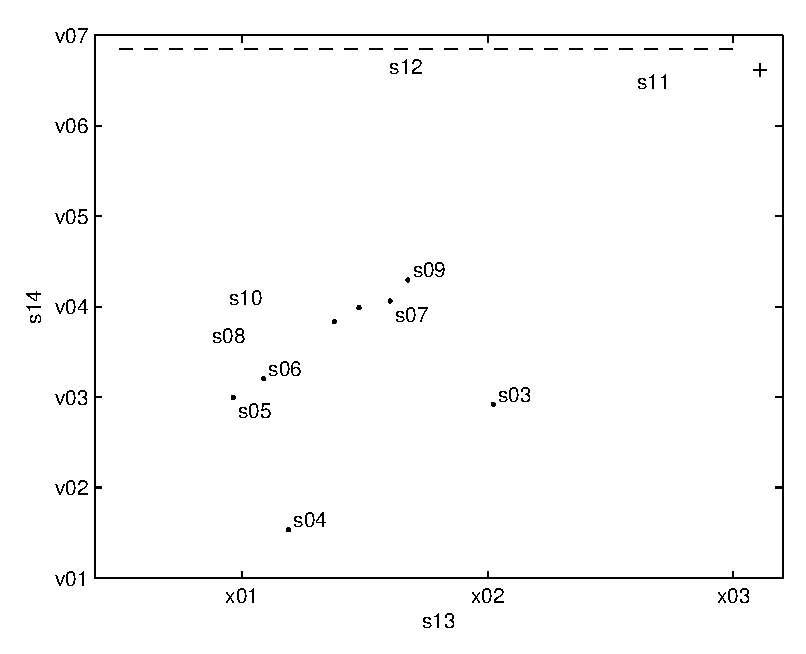
\includegraphics{Psaltis_plot.eps}}%
\end{psfrags}%
%
% End Psaltis_plot.tex
\end{document}
% See http://www.mathworks.de/matlabcentral/fileexchange/loadFile.do?objectId=4638
% for recent versions of laprint.m.
%
% created by:           LaPrint version 3.16 (13.9.2004)
% created on:           31-Jul-2013 16:31:14
% eps bounding box:     15 cm x 11.25 cm
% comment:              
%
\begin{psfrags}%
\psfragscanon%
%
% text strings:
\psfrag{s03}[l][l]{\color[rgb]{0.83529,0.36863,0}\setlength{\tabcolsep}{0pt}\begin{tabular}{l}$10^6 M_\odot$\end{tabular}}%
\psfrag{s04}[l][l]{\color[rgb]{0.83529,0.36863,0}\setlength{\tabcolsep}{0pt}\begin{tabular}{l}$M_\odot$\end{tabular}}%
\psfrag{s05}[l][l]{\color[rgb]{0.83529,0.36863,0}\setlength{\tabcolsep}{0pt}\begin{tabular}{l}$M_\oplus$\end{tabular}}%
\psfrag{s06}[l][l]{\color[rgb]{0,0.44706,0.69804}\setlength{\tabcolsep}{0pt}\begin{tabular}{l}$1~\mathrm{m}$\end{tabular}}%
\psfrag{s07}[l][l]{\color[rgb]{0,0.44706,0.69804}\setlength{\tabcolsep}{0pt}\begin{tabular}{l}$10~\mathrm{km}$\end{tabular}}%
\psfrag{s08}[l][l]{\color[rgb]{0,0.44706,0.69804}\setlength{\tabcolsep}{0pt}\begin{tabular}{l}$1 R_\oplus$\end{tabular}}%
\psfrag{s09}[l][l]{\color[rgb]{0,0.44706,0.69804}\setlength{\tabcolsep}{0pt}\begin{tabular}{l}$1 R_\odot$\end{tabular}}%
\psfrag{s10}[l][l]{\color[rgb]{0,0.44706,0.69804}\setlength{\tabcolsep}{0pt}\begin{tabular}{l}$1~\mathrm{mpc}$\end{tabular}}%
\psfrag{s11}[l][l]{\color[rgb]{0,0,0}\setlength{\tabcolsep}{0pt}\begin{tabular}{l}GP-B\end{tabular}}%
\psfrag{s12}[l][l]{\color[rgb]{0,0,0}\setlength{\tabcolsep}{0pt}\begin{tabular}{l}LLR (Earth--Moon)\end{tabular}}%
\psfrag{s13}[l][l]{\color[rgb]{0,0,0}\setlength{\tabcolsep}{0pt}\begin{tabular}{l}LLR (Earth--Moon--Sun)\end{tabular}}%
\psfrag{s14}[l][l]{\color[rgb]{0,0,0}\setlength{\tabcolsep}{0pt}\begin{tabular}{l}Mercury\end{tabular}}%
\psfrag{s15}[l][l]{\color[rgb]{0,0,0}\setlength{\tabcolsep}{0pt}\begin{tabular}{l}Cassini\end{tabular}}%
\psfrag{s16}[l][l]{\color[rgb]{0,0,0}\setlength{\tabcolsep}{0pt}\begin{tabular}{l}Hulse--Taylor\end{tabular}}%
\psfrag{s17}[l][l]{\color[rgb]{0,0,0}\setlength{\tabcolsep}{0pt}\begin{tabular}{l}J0348+0432\end{tabular}}%
\psfrag{s18}[l][l]{\color[rgb]{0,0,0}\setlength{\tabcolsep}{0pt}\begin{tabular}{l}Double pulsar\end{tabular}}%
\psfrag{s19}[l][l]{\color[rgb]{0,0,0}\setlength{\tabcolsep}{0pt}\begin{tabular}{l}Neutron star\end{tabular}}%
\psfrag{s20}[l][l]{\color[rgb]{0,0,0}\setlength{\tabcolsep}{0pt}\begin{tabular}{l}Black holes\end{tabular}}%
\psfrag{s21}[t][t]{\color[rgb]{0,0,0}\setlength{\tabcolsep}{0pt}\begin{tabular}{c}{\Large{$\xi/\mathrm{m^{-2}}$}}\end{tabular}}%
\psfrag{s22}[b][b]{\color[rgb]{0,0,0}\setlength{\tabcolsep}{0pt}\begin{tabular}{c}{\Large{$\varepsilon$}}\end{tabular}}%
%
% xticklabels:
\psfrag{x01}[t][t]{$10^{-30}$}%
\psfrag{x02}[t][t]{$10^{-25}$}%
\psfrag{x03}[t][t]{$10^{-20}$}%
\psfrag{x04}[t][t]{$10^{-15}$}%
\psfrag{x05}[t][t]{$10^{-10}$}%
%
% yticklabels:
\psfrag{v01}[r][r]{$10^{-12}$}%
\psfrag{v02}[r][r]{$10^{-10}$}%
\psfrag{v03}[r][r]{$10^{-8}$}%
\psfrag{v04}[r][r]{$10^{-6}$}%
\psfrag{v05}[r][r]{$10^{-4}$}%
\psfrag{v06}[r][r]{$10^{-2}$}%
\psfrag{v07}[r][r]{$10^{0}$}%
%
% Figure:
\resizebox{12cm}{!}{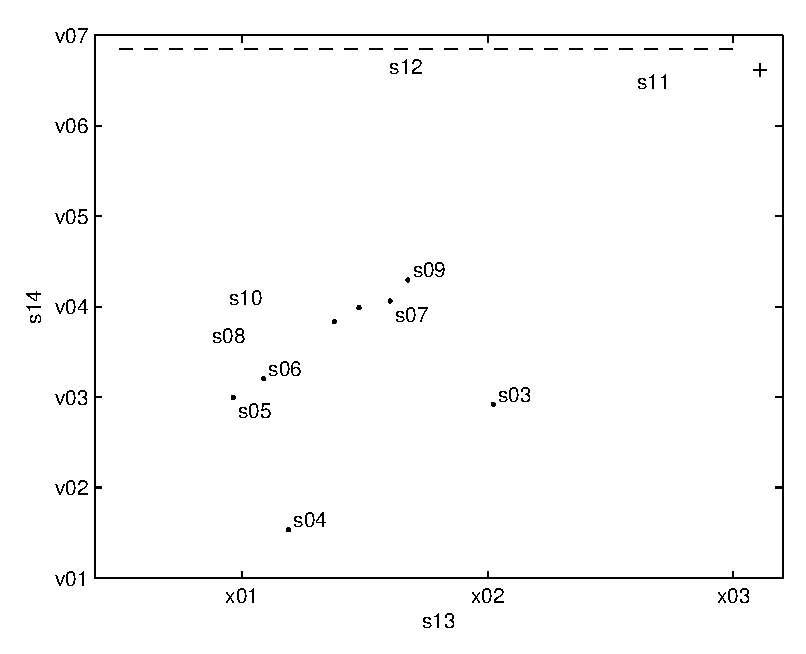
\includegraphics{Psaltis_plot.eps}}%
\end{psfrags}%
%
% End Psaltis_plot.tex
\end{document}
% See http://www.mathworks.de/matlabcentral/fileexchange/loadFile.do?objectId=4638
% for recent versions of laprint.m.
%
% created by:           LaPrint version 3.16 (13.9.2004)
% created on:           03-Aug-2013 13:00:27
% eps bounding box:     15 cm x 11.25 cm
% comment:              
%
\begin{psfrags}%
\psfragscanon%
%
% text strings:
\psfrag{s03}[l][l]{\color[rgb]{0.83529,0.36863,0}\setlength{\tabcolsep}{0pt}\begin{tabular}{l}$10^6 M_\odot$\end{tabular}}%
\psfrag{s04}[l][l]{\color[rgb]{0.83529,0.36863,0}\setlength{\tabcolsep}{0pt}\begin{tabular}{l}$M_\odot$\end{tabular}}%
\psfrag{s05}[l][l]{\color[rgb]{0.83529,0.36863,0}\setlength{\tabcolsep}{0pt}\begin{tabular}{l}$M_\oplus$\end{tabular}}%
\psfrag{s06}[l][l]{\color[rgb]{0,0.44706,0.69804}\setlength{\tabcolsep}{0pt}\begin{tabular}{l}$1~\mathrm{m}$\end{tabular}}%
\psfrag{s07}[l][l]{\color[rgb]{0,0.44706,0.69804}\setlength{\tabcolsep}{0pt}\begin{tabular}{l}$10~\mathrm{km}$\end{tabular}}%
\psfrag{s08}[l][l]{\color[rgb]{0,0.44706,0.69804}\setlength{\tabcolsep}{0pt}\begin{tabular}{l}$1 R_\oplus$\end{tabular}}%
\psfrag{s09}[l][l]{\color[rgb]{0,0.44706,0.69804}\setlength{\tabcolsep}{0pt}\begin{tabular}{l}$1 R_\odot$\end{tabular}}%
\psfrag{s10}[l][l]{\color[rgb]{0,0.44706,0.69804}\setlength{\tabcolsep}{0pt}\begin{tabular}{l}$1~\mathrm{mpc}$\end{tabular}}%
\psfrag{s11}[l][l]{\color[rgb]{0,0,0}\setlength{\tabcolsep}{0pt}\begin{tabular}{l}GP-B\end{tabular}}%
\psfrag{s12}[l][l]{\color[rgb]{0,0,0}\setlength{\tabcolsep}{0pt}\begin{tabular}{l}LLR (Earth--Moon)\end{tabular}}%
\psfrag{s13}[l][l]{\color[rgb]{0,0,0}\setlength{\tabcolsep}{0pt}\begin{tabular}{l}LLR (Earth--Moon--Sun)\end{tabular}}%
\psfrag{s14}[l][l]{\color[rgb]{0,0,0}\setlength{\tabcolsep}{0pt}\begin{tabular}{l}Mercury\end{tabular}}%
\psfrag{s15}[l][l]{\color[rgb]{0,0,0}\setlength{\tabcolsep}{0pt}\begin{tabular}{l}Cassini\end{tabular}}%
\psfrag{s16}[l][l]{\color[rgb]{0,0,0}\setlength{\tabcolsep}{0pt}\begin{tabular}{l}Hulse--Taylor\end{tabular}}%
\psfrag{s17}[l][l]{\color[rgb]{0,0,0}\setlength{\tabcolsep}{0pt}\begin{tabular}{l}J0348+0432\end{tabular}}%
\psfrag{s18}[l][l]{\color[rgb]{0,0,0}\setlength{\tabcolsep}{0pt}\begin{tabular}{l}Double pulsar\end{tabular}}%
\psfrag{s19}[l][l]{\color[rgb]{0,0,0}\setlength{\tabcolsep}{0pt}\begin{tabular}{l}Neutron star\end{tabular}}%
\psfrag{s20}[l][l]{\color[rgb]{0,0,0}\setlength{\tabcolsep}{0pt}\begin{tabular}{l}Black holes\end{tabular}}%
\psfrag{s21}[t][t]{\color[rgb]{0,0,0}\setlength{\tabcolsep}{0pt}\begin{tabular}{c}{\Large{$\xi/\mathrm{m^{-2}}$}}\end{tabular}}%
\psfrag{s22}[b][b]{\color[rgb]{0,0,0}\setlength{\tabcolsep}{0pt}\begin{tabular}{c}{\Large{$\varepsilon$}}\end{tabular}}%
%
% xticklabels:
\psfrag{x01}[t][t]{$10^{-30}$}%
\psfrag{x02}[t][t]{$10^{-25}$}%
\psfrag{x03}[t][t]{$10^{-20}$}%
\psfrag{x04}[t][t]{$10^{-15}$}%
\psfrag{x05}[t][t]{$10^{-10}$}%
%
% yticklabels:
\psfrag{v01}[r][r]{$10^{-12}$}%
\psfrag{v02}[r][r]{$10^{-10}$}%
\psfrag{v03}[r][r]{$10^{-8}$}%
\psfrag{v04}[r][r]{$10^{-6}$}%
\psfrag{v05}[r][r]{$10^{-4}$}%
\psfrag{v06}[r][r]{$10^{-2}$}%
\psfrag{v07}[r][r]{$10^{0}$}%
%
% Figure:
\resizebox{12cm}{!}{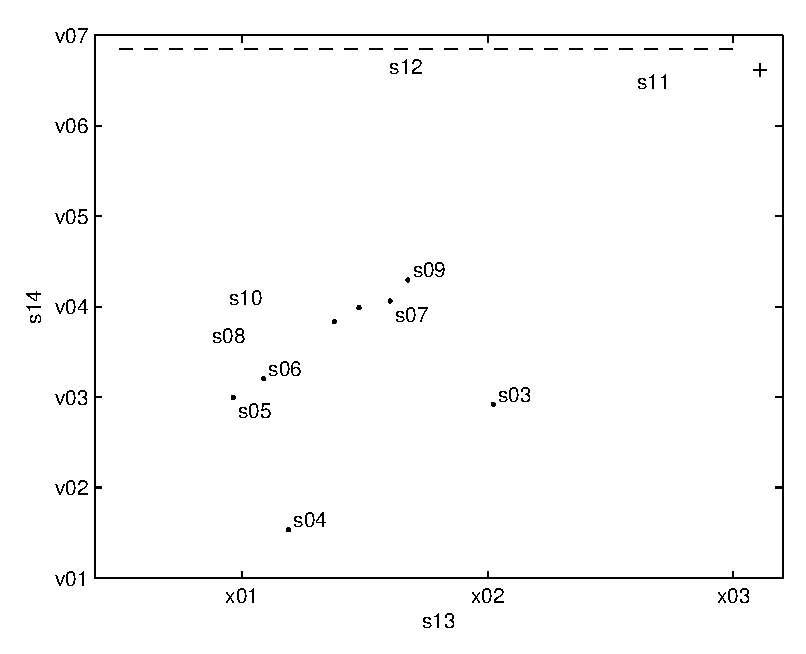
\includegraphics{Psaltis_plot.eps}}%
\end{psfrags}%
%
% End Psaltis_plot.tex
